\documentclass{article}
\usepackage{fullpage}
\usepackage[utf8]{inputenc}
\usepackage[title]{appendix}
\usepackage{amsmath}
\usepackage{amssymb}
\usepackage{amsthm}
\usepackage{url}
\usepackage{tabularx}
\usepackage{floatrow}
\usepackage{graphicx}
\usepackage{subcaption}
\graphicspath{ {./images/} }

\floatsetup{heightadjust=object}

\newcommand{\figref}[1]{Figure \ref{#1}}
\newcommand{\tabref}[1]{Table \ref{#1}}
\newcommand{\secref}[1]{Section \ref{#1}}
\newcommand{\apdxref}[1]{Appendix \ref{#1}}

\newcommand{\CH}{\mathrm{CH}}
\newfloatcommand{capbtabbox}{table}[][\FBwidth]

\title{An Implementation Analysis of the \\ $O(n \log^4 n)$ Minimum Perimeter-Sum Bipartition Algorithm}
\author{Allen Mi, Haakon Flatval}
\date{December 2018}

\begin{document}

\maketitle

\begin{abstract}
    The minimum perimeter-sum bipartition problem is stated as follows: Given set of points in the Euclidean plane, partition it into two subsets such that the sum of perimeters of their convex hulls is as small as possible. In this report, we describe the algorithm by Abrahamsen et al. \cite{abb17}, and identify the structural hierarchy of its subroutines. We compare the empirical running time of select subroutines with their theoretical bounds. We analyze the performance bottlenecks of the algorithm, and identify the characteristics of worst-case inputs. Finally, we discuss the limitations of our work and the difficulties in bringing the algorithm to a practical domain.
    % Is this too harsh on us? yes lol. Nice. Looks good to me
    % Fill in more here / rewrite abstract as things happen
\end{abstract}

\section{Introduction}
The minimum perimeter-sum bipartition problem is the problem of partitioning a set of points in the two-dimensional plane into two disjoint subsets $P_1$ and $P_2$ such that the sum of the perimeters of $\text{CH}(P_1)$ and $\text{CH}(P_2)$ is minimized, where $\text{CH}(P)$ is the convex hull of the set of points $P$. In 2017, Abrahamsen et al. \cite{abb17} devised an algorithm that solves this problem in time $O(n \log^4 n)$, $n$ being the number of points in the input.

\subsection{The Scope of this Project}

Our goal is to analyze the structure of the algorithm presented in \cite{abb17}, identify its performance bottleneck, and find characteristics of adversarial inputs.

We do not provide a full implementation of the algorithm. Instead, we focus on the subroutines that have the greatest impact on the running time. For these subroutines, we compare their empirical running times and theoretical bounds.

We are not able to implement an important subroutine for combining convex hulls within the specified time bound. We have not been able to identify a way that allows us to withhold this bound in practice. We will briefly discuss the issue by the end of this report.

Our implementation is completed in \texttt{C++}. The codebase is publicly available at \cite{hm18}.

\subsection{The Structure of this Report}

A formal definition of the minimum perimeter-sum bipartition problem is introduced in \secref{sec:background}, alongside a detailed review of the algorithm. A summary of the algorithm is presented in \ref{sub:summary_of_algorithm}. Details of our implementation is available at \secref{sec:implementation}, with an illustration of the algorithm's structural hierarchy at \figref{fig:hierarchy}. \secref{sec:performance_and_input_design} is dedicated to evaluating and analyzing the algorithm's performance. Empirical results of select subroutines are discussed in \ref{sub:empirical_running_times}. The performance bottleneck of the algorithm is discussed in \ref{sub:designing_adversarial_inputs}, where the characteristics of adversarial inputs are also discussed. \secref{sec:limitations} discusses the practical limitations of the algorithm, as well as the aspects not covered by this project. Finally, \secref{sec:conclusion} provides a conclusion of our project.

\section{Background} \label{sec:background}

% Description of the problem and the algorithm

We here walk through the algorithm solving the minimum perimeter-sum bipartition problem.

Abrahamsen et al. \cite{abb17} shows that, for any optimal partition $\{P_1^*, P_2^*\}$ of the input points, the following holds:

\textit{Either the outer angle between the inner tangents of the convex hulls
$\text{CH}(P_1^*)$ and $\text{CH}(P_2^*)$ (see illustration) is at least $\pi / 6$, or the smallest distance between two
points in $P_1^*$ and $P_2^*$ is at least $1/250 \cdot \min(\text{per}(P_1^*), \text{per}(P_2^*))$}. 

$\text{per}(P)$ denotes the length of the perimeter of the convex hull of $P$. In figure \figref{fig:tangent_angle}, we show the two inner tangents of two polygons $L_1$ and $L_2$ of the polygons, with the outer angle $B$ in-between them.

In the remainder of the discussion, the angle $B$ is referred to as the separation angle.

This immediately splits our approach into two cases, one where we assume the separation angle to be at least $\pi / 6$, and another where we assume the distance between the sets to be "large". 


We solve the problem with each of these assumptions in turn, and choose the best of the results as our answer.


\begin{figure}[ht]
    \centering
    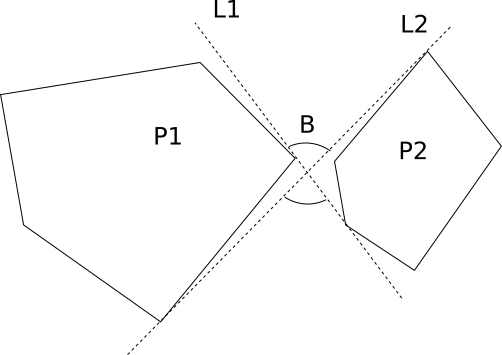
\includegraphics[width=0.5\textwidth]{images/inner_angle.png}
    \caption{The inner tangents $L_1$ and $L_2$ and their outer angle $B$}
    \label{fig:tangent_angle}
\end{figure}


\subsection{Algorithm Assuming Large Separation Angle of Solution}

In the case where the separation angle is larger than $\pi / 6$, we make the following observation: Consider the set of seven angles $\Phi = \{\pi \cdot i / 7 \,  | \, i \in [0, 7) \}$. There must exist a line separating the optimal subsets, whose angle is among those seven. Thus, we will approach as follows:

For each of the angles $\phi \in \Phi$, we use a line $l_\phi$ having angle $\phi$ in a Graham's scan; that is, we treat $l_\phi$ as a scanning line in a modified version of Graham's algorithm: When first scanning from one side to the other, we compute the "upper" hull, as usual, but we also make sure to store the length of the upper hull ending at each intermediate point. The same is done for the the lower hull when scanning the other way, and the process is repeated switching the direction of scan for upper and lower hull. 

Now, each point has four lengths associated with it (from being the end point for the upper and lower hull from each of the two scanning directions), which makes it easy for us to compute the total length of any convex hull ending at each point in constant time. Scanning through the points again, repeatedly using the two points immediately to each side of the scanning line and computing the length two hulls ending at these points, we can find the best possible partition with separating line of angle $\phi$.

Repeating this approach for each of the seven angles, we will, by assumption of large separation angle, find the best partition overall.

This approach uses Graham's algorithm a constant number of times, and thus has a complexity of $O(n \log n)$.

\subsection{Algorithm Assuming Large Separation Distance of Solution}

Now, we must find the best possible partition assuming the distance between the two subsets is large. 

We first treat the special case where one of the subsets is a single point $p$. Some thought reveal that $p$ must lie on the convex hull of the set of input points $P$. We will thus go through each of the points $v_i$ at the boundary of $\text{CH}(P)$ in turn and compute the perimeter $\text{per}(P \setminus \{v_i\}$. 

We do this by constructing each triangle $\Delta_i$ formed by three consecutive points on the boundary $v_{i - 1}$, $v_i$ and $v_{i + 1}$, and find the set $P_i$ of the points contained inside $\Delta_i$, excluding $v_i$, but including $v_{i - 1}$ and $v_{i + 1}$. Note now that each point can belong to a maximum of two triangles. According to $\cite{abb17}$, doing this is "easy" in $O(n \log n)$ time, without specifying how. We have chosen to compute the set $P_i$ in the following way:
\begin{itemize}
    \item Construct a suitable center point $c$ not contained in any triangle \textit{We find this by taking the crossing between two diagonals}
    \item Sort the points by their angle around the center point, such that a chosen first boundary point $v_0$ has angle $0$
    \item Initialize $t_0 = \Delta_0$, $t_1 = \Delta_1$
    \item Iterate over each point $p_i$: \begin{itemize}
        \item If $p_i$ is the end point of $t_0$, shift $t_0$ and $t_1$ to the next $\Delta$
        \item If $p_i$ is inside $t_0$ or $t_1$ (or both), put it in the triangle's respective set
    \end{itemize}
\end{itemize}

Finally, having found the sets $P_i$, we compute the convex hulls $\text{CH}(P_i)$, and can find the perimeters $\text{per}(P \setminus \{v_i\})$ as $\text{per}(P \setminus \{v_i\}) = \text{per}(P) - |v_{i - 1}v_i| - |v_iv_{i + 1}| + \text{per}(P_i) - |v_{i - 1}v_{i + 1}|$.

Thus, finding the optimal partition where one of the sets is a single point, can be done in $O(n \log n)$ time.

Now we have reduced the problem to the following: Partition the set $P$ into two non-trivial sets with smallest sum of perimeters. 

$\cite{abb17}$ proceeds at this point to compute a set $S$ of $O(n)$ axis-aligned squares which is certain to contain a so-called \textit{good} square,  a square in the plane that fully contains one of the optimal subsets, and such that one edge of the square is no longer than 18 times the perimeter of that optimal subset.

We will not go into detail as to how the set $S$ is computed, as the technique uses a compressed quad tree \cite{quad_trees}, which is well beyond what there is room for here given reasonable prerequisites. We also find this computation unlikely to be a bottleneck for our analysis, as its constant factor is (relatively) low and the algorithm runs in $O(n \log n)$ time. For the remainder of this discussion, we will assume that we have found the set $S$ of squares, among which at least one is \textit{good}.

What we will do in the following, is to intersect each of the $O(n)$ square $\sigma_i$ in $S$ with a constant number of lines $l_j$, each line representing the boundary of a half plane $h_j$. For each such half plane, we will find the set of points within the square, and also within the half plane: $P \cap \sigma_i \cap h_j$. 

From the way we construct these half planes (which we will review shortly), and from the assumption of large separation distance, if $\sigma_i$ is a good square, the set $P \cap \sigma_i \cap h_j$ will be one of the optimal sets for some half plane $h_j$ (Lemma 8 in \cite{abb17}). We will thus compute all such intersections of a half plane and a square, and pick the one optimizing the perimeter lengths. The remainder of this section will assess how we proceed to compute these set intersections and the corresponding perimeter lengths.

The half planes are constructed as follows: $4 \cdot 18 / \dfrac{1}{250} + 1 = 18001$ points are placed evenly around the perimeter of the square. The number is chosen such that the distance between two neighboring points is less than the separation distance between the optimal sets, if one of the sets is contained within the square. Now, we create the set of lines connecting every pair of these points. We thus create a set of $O(18001^2)$ lines, which are the boundaries of the half planes $h_j$.

The next question we have to answer, is how to find the set $P \cap \sigma_i \cap h_j$, and also $\text{per}(P \cap \sigma_i \cap h_j)$ fast. Notice that this is a query for a set of points in a rectangular axis-align region, then cut against a half plane. A normal two-level range tree \cite{range_trees} can be used for query for sets contained in axis-align rectangles, and adding one more level to the range tree for the half plane axis (perpendicular to the half plane boundary) ensures that we can now also easily find a set of points on a specific side of the half plane. 

Thus, for each of the half planes constructed, we also construct a range tree. Now, note that for any square, all the lines we constructed for that square will have its counterpart lines in other squares with the same angle and relative placement within the square. Since the sorting of the lowest level of the range tree will only depend on the angle of the respective half plane, we will only need to construct a constant number of range trees, one for each half plane angle. 

As mentioned, when finding the set $P \cap \sigma_i \cap h_j$ with a range tree query, we are also interested in finding its perimeter. We can do this by augmenting each node of the lowest level trees in the range tree to contain the convex hull of all nodes in the subtree rooted at that node. This can be done recursively, in the sense that the convex hull of a node can be computed by combining the hulls at its two children. We have implemented this by computing the outer tangents (so that the two polygons lie on the same side of each tangent) using \cite{ks95}, and their touch points on both polygons, and tracing the original hulls, but upon hitting a touch point, switches to the corresponding touch point of the other polygon. We remark that \cite{ks95} directly computes the touch point indices in the polygons, and not the tangent lines themselves.

This construction gives us a range tree that contains convex hulls at its nodes in $O(n \log^3 n)$ time and using $O(n \log^3 n)$ space. Now. a general query region of the form $\sigma_i \cap h_j$ will in $O(\log^3n)$ time return $O(\log^3 n)$ nodes from the range tree, each covering a disjoint subset of the points in the query region. We will also make a few more disjoint queries into the range tree, in order to find $P \setminus (\sigma_i \cap h_j)$. We will need up to five more queries of the same form as the first. 

Now we have found a candidate partition, the set of points within $\sigma_i \cap h_j$ and the set of points outside. We have now a collection of $O(\log^3 n)$ convex hulls representing each of the region. In the last part of this section, we show how to compute the combined hull and perimeter length of each of those collections. 

The general approach to combine a set of convex hulls into one, is to scan over them using Graham's scan. Before doing so, however, we first construct a new set of polygons in the following way: Create two "events" for each polygon, one corresponding to its first (leftmost) point, and the second to its last point (rightmost) point. Sort this list, and traverse it. Imagine this as a scan line scanning over the polygons left to right. We keep track of all the currently "active" polygons in a balanced binary tree (e.g. a red-black tree), sorted on their y-coordinate (which is well defined between "active" polygons, as the they are disjoint). Whenever the scan line hits a new polygon, it is inserted in the tree, and likewise deleted when the scan line passes it. Whenever the top node changes, (and the tree was non-empty before the change), a polygon is constructed by taking a vertical slice of the previous top polygon from this point of change to the previous point of change. Doing this until the scan line has passed all polygons, we have created a new set of polygons, each occupying disjoint ranges in the x-axis. Figure \ref{fig:vertical_slices} shows an example of the result of this process.

\begin{figure}
    \centering
    \begin{subfigure}[b]{0.4\textwidth}
    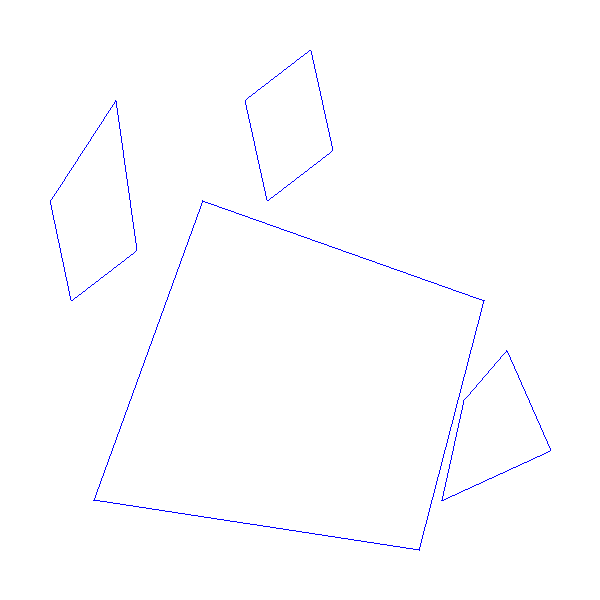
\includegraphics[width=\textwidth]{images/before_new_polygons.png}
    \end{subfigure}
    %
    \begin{subfigure}[b]{0.4\textwidth}
    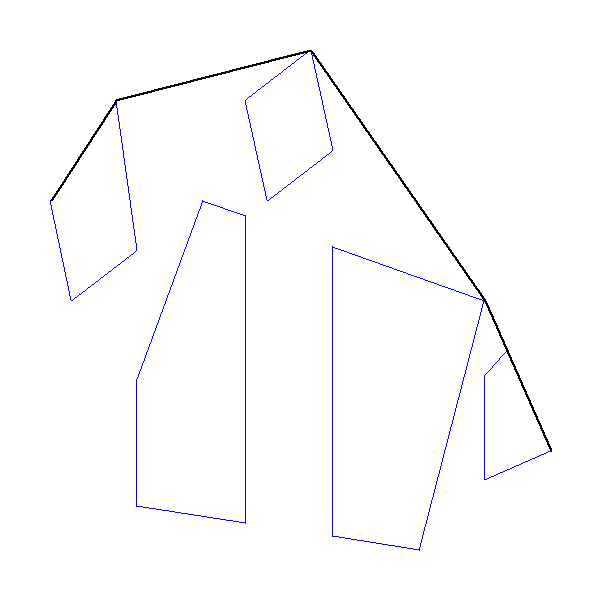
\includegraphics[width=\textwidth]{images/new_polygons_with_half_hull.png}
    \end{subfigure}
    \caption{Left: The original convex hulls we want to combine to one hull. Right: The new polygons, constructed as vertical slices of the original polygons, disjoint on the x-axis. The thick line is the upper half of the resulting convex hull}
    \label{fig:vertical_slices}
\end{figure}

Now, we will run something very similar to a Graham's scan, going through the polygons from left to right, an ordering that is now well defined. When considering a new polygon to add to the hull, we check the (upper, outer) tangent between the two previous polygons and the one between the previous polygon and the new one, using the tangent algorithm in \cite{ks95}. We compare these two tangents, if they make a right turn, we add the new polygon in our list. If not, we discard the last polygon  already added, and try inserting the new polygon again.

In the end, having determined which polygons belong to the hull and not, we find the hull length itself using the point indices given to us by the tangent computation. Note that we here only have described how to compute the length of the upper part of the hull. Computing the length of the lower part is analogous. 

The paper \cite{abb17} describes this algorithm to take $k \log m$ time, $k$ being the number of hulls, $m$ the total number of points in the hulls. Thus, since we will use this procedure on sets containing at most $O(\log^3 n)$ hulls, we can conclude that each such "hull combining call" takes time $O(\log^4 n)$.

\subsection{Summary of Algorithm} \label{sub:summary_of_algorithm}

For convenience, we summarize the main steps of the algorithm here. The highest level view is that we compute many candidate solutions and pick the best one. We compute the candidate solutions in the following ways:

\begin{itemize}
    \item Do several Graham scans in seven different directions, to find the best bipartition with separation angle greater than $\pi / 6$.
    \item Compute set of points contained in each triangle formed by three consecutive points on the convex hull $\text{CH}(P)$ of all input points, and use this to compute length of the convex hull of $P \setminus v_i$ for each corner $v_i$ of $\text{CH}(P)$. This finds the best partition where one of the sets is trivial.
    \item Construct $O(n)$ squares, and intersect each of them with $O(1)$ lines. Precompute $O(1)$ three-level range trees searchable in x- and y-axis and in the direction perpendicular to one of the $O(1)$ lines. For each square and each line (we think of each line as two complementary half planes), find the set of points in the intersection of the square and the half plane by a query into the appropriate range tree, and similarily, find the rest of the points in $P$ by more queries, retrieving $O(\log^3 n)$ hulls. Combine the hulls belonging to each of these two sets in $O(\log^4)$ time, and find their lengths. This finds the best partition where the sets have a "large" separation distance.
\end{itemize}

The outline of the program flow is show in \figref{fig:hierarchy}.

\section{Implementation} \label{sec:implementation}

\subsection{Perturbation}

As a preprocessing step of our input points, we perform an operation inspired by \textit{symbolic perturbation} \cite{edelsbrunner90} on the input points. 

We want to avoid degeneracies in our input set. That is, we want to avoid having three distinct point lying on the same line. Such colinear points form special edge cases to several of our algorithms, which would increase the complexity of our implementation significantly. 

We have chosen a very simple approach to address this that has worked well in our analysis. Each point $p_i$ is displaced by a small vector $\epsilon_i$ drawn from a normal distribution. Note that the sum of perimeters of the optimal bipartition cannot change by more than a constant times $\max |\epsilon_i|$, and that the difference of the sum of perimeters in an optimal partition and a suboptimal one is non-infinitesimal. This means that choosing $\epsilon_i$ small enough will ensure that the optimal bipartition we find is indeed optimal when using the original coordinates of the points as well.

Naturally, this step is not a deterministic solution to the problem of degeneracy, but suffices in our analysis under controlled conditions. Real implementations would do wisely in making this process deterministic.

\subsection{Hierarchy of Subroutines}

Here follows a description of the most important subroutines of the algorithm. Refer to figure \ref{fig:hierarchy} for an overview of the relations between them. 

% Dependency information of the subroutines
\begin{figure}[ht]
    \centering
    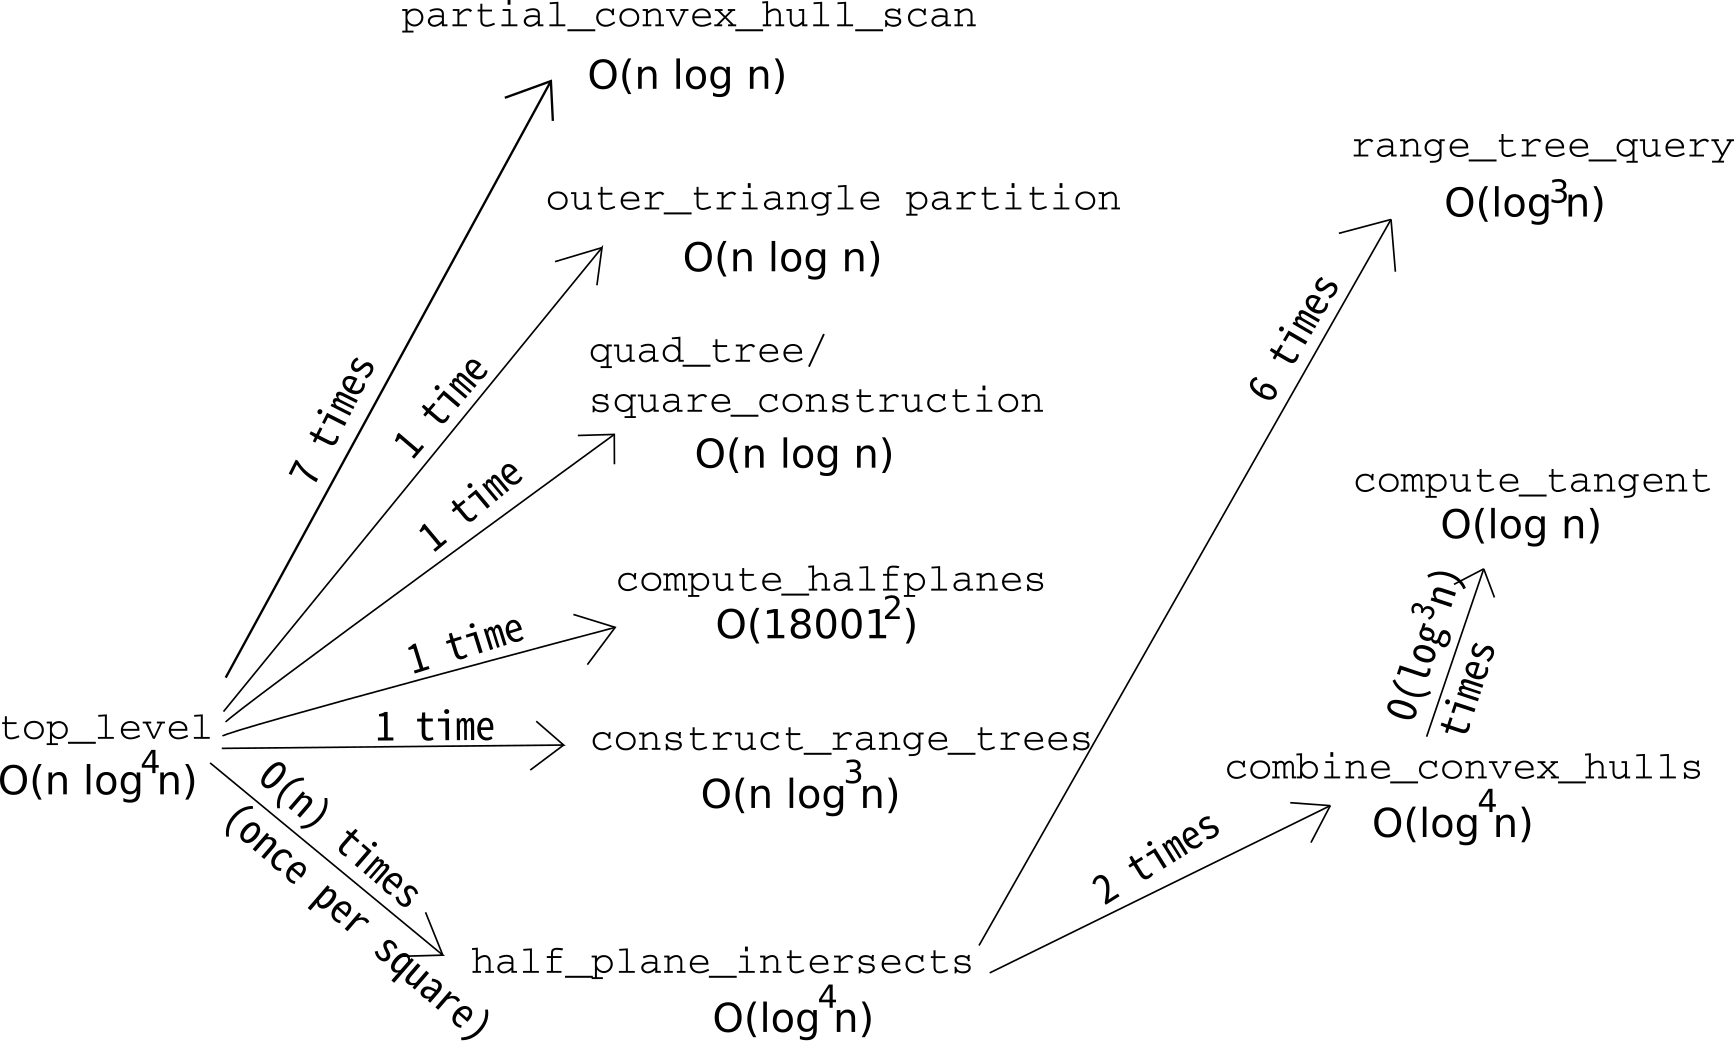
\includegraphics[width=0.75\textwidth]{hierarchy.png}
    \caption{Structural hierarchy of subroutines. The complexity of each subroutine is denoted under their name. The arrows show which subroutines call which others, and how many times per call to themselves.}
    \label{fig:hierarchy}
\end{figure}

\subsubsection{Partial Convex Hull Scan}

For a given angle $\phi$ and a set of points $P$, this subroutine computes the upper and lower halves of the convex hull of $P$, scanning through the nodes like in Graham's scan, but along a line with angle $\phi$ to the x-axis. This allows us to quickly compute convex hulls of a bipartition of $P$ separated by a line perpendicular to the scan direction. This operation takes $O(n \log n)$ time for a given angle, $n$ being the size of $P$.

\subsubsection{Outer Triangle Partitioning} \label{subsub:outer_triangle_partitioning}

For a given set of points $P$, computes all triangles formed by three successive points on the set's convex hull, and finds and stores the subset of the points contained in each such triangle. This allows us to quickly compute the length of the convex hull of $P \setminus {p}$, where $p$ is a point on the convex hull of $P$. This operation takes $O(n \log n)$ time, where $n = |P|$.
    
\subsubsection{Quad Tree Construction} 

Each node in such a quad tree represents a square in the plane. Each node has four children, representing the regions of the four equal squares that make up their parent's region. The construction of a compressed quad tree over $n$ points takes $O(n \log n)$ time, given an appropriate computational model is used.

\subsubsection{Range Tree Construction and Search} \label{subsub:range_tree_construction_and_search}

The range tree we construct here has three levels. The first level sorts the points on the x-axis, the subsequent level sorts the points at each node by the y-axis. The lowest level sort the points by a given direction in the plane. This allows us to easily find points that are restricted to a given rectangular axis-aligned region in the plane, and that are also inside a specified half-plane. This range tree also compute the convex hull of each node in the lowest level of the range tree. The range tree construction takes $O(n\log^3n)$, $n$ being the number of points over which we construct the tree.

\subsubsection{Tangent Computation} \label{subsub:tangent_computation}

For two polygons $A$ and $B$, computes their tangents using the algorithm provided in \cite{ks95}. We use this to determine which polygons belongs to the hull in the \textit{convex hull combining} subroutine. The algorithm uses $O(\log(a + b))$ time, where $a$ and $b$ are the number of points on the boundary of $A$ and $B$ respectively.

\subsubsection{Convex Hull Combining}
For a given set of convex hulls $\mathcal{C}$, finds the convex hull of all points on all the hulls. We use this to combine the convex hulls found from a query in the range tree described above, including its length, so that we can evaluate the perimeter. The running time for this subroutine is $O(k \log m)$, $k$ being the number of convex polygons, and $m$ the number of points on the hulls in total.

\subsection{Choosing Subroutines to Implement}

As mentioned in the introduction, we have decided to only implement a subset of the subroutines. The subroutines we have decided to cover are: \texttt{construct\_range\_tree(s)}, \texttt{range\_tree\_query}, and \texttt{combine\_convex\_hull}. In addition, we have included the implementation of \texttt{compute\_tangent} directly adapted from \cite{ks95}, as this serves as a component to other subroutines. 

We have chosen these subroutines because their individual performances are likely to have a significant impact on the total performance in practice. This conclusion is drawn on the basis of their importance in the structural hierarchy: they either are required by a number of other subroutines, or run a large constant number of times, in the order of $18001^2$.

We also provide an implementation and analysis of \texttt{outer\_triangle\_partition}, as we found ourselves curious with how this algorithm of our own design would perform. % Or do we? Is it useful?
% Should we provide analysis for the outer_triangle_partition subroutine?

\newpage

\section{Performance and Input Design} \label{sec:performance_and_input_design}

% Performance analysis of each subroutine, as well as the entire algorithm. The sample input of the performance analysis could be from uniform sampling of the target rectangular region.

\subsection{Empirical Running Times} \label{sub:empirical_running_times}

Recall from \figref{fig:hierarchy} the structural hierarchy of this algorithm. We are mainly interested in the leaf entries of the dependency tree, as they constitute the basic subroutines of the algorithm. In this section, we perform empirical performance testing on the basic subroutines we have implemented, and discuss the relationship between the theoretical bounds outlined in \cite{abb17} and our empirical results. We primarily investigate how their running times scale with respect to the size of input. The detailed hardware specifications and testing methodology are listed in \apdxref{apdx:specifications}.

\subsubsection{Outer Triangle Partitioning}

The outer triangle partitioning, as described in \ref{subsub:outer_triangle_partitioning}, is an $O(n \log n)$ operation, where $n$ denotes the size of the input set of points. The outer triangle partitioning is tested on point sets of size $n = 10^4 k + 1$ for each $k \in [0, 9]$. For each $k$, the set of points is generated by taking $n$ random samples of the unit disk under uniform distribution. The results are presented in \figref{fig:outer_triangle_partition_performance}. We derive a line of best fit $y = \alpha(n \log n) + \beta$ with $\alpha = 6.142 \times 10^{-4}$ and $\beta = -9.784 \times 10^{-1}$. This gives an empirical complexity of $t \sim 6.142 \times 10^{-4} n \log n -9.784 \times 10^{-1}$, where $t$ denotes the running time. The empirical running time matches the theoretical bound of $O(n \log n)$.

\begin{figure}[h!]
    \begin{floatrow}
        \ffigbox[\FBwidth][\FBheight][t]{
            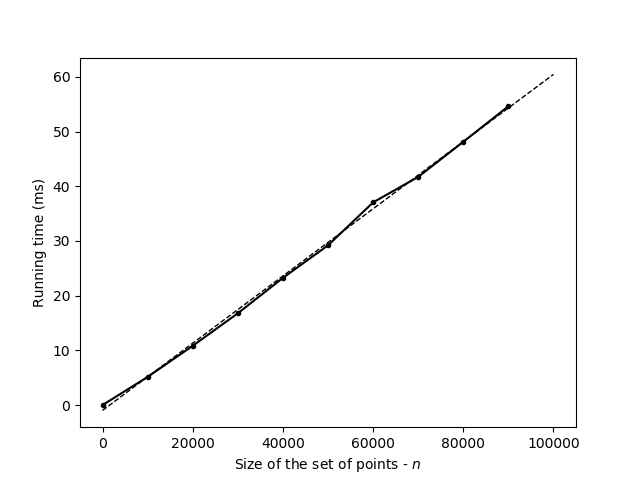
\includegraphics[width=0.6\textwidth]{outer_triangle_partition_performance}
        }{
            \caption{Performance of the outer triangle partitioning}
            \label{fig:outer_triangle_partition_performance}
        }
        \capbtabbox[0.3\textwidth][\FBheight][t]{
            \small
            \begin{tabular}{cc}
                Size $n$ & Running time (ms) \\
                \hline
                $1$ & 0.002 \\
                $10001$ & 5.145 \\
                $20001$ & 10.831 \\
                $30001$ & 16.776 \\
                $40001$ & 23.247 \\
                $50001$ & 29.197 \\
                $60001$ & 37.049 \\
                $70001$ & 41.707 \\
                $80001$ & 48.124 \\
                $90001$ & 54.627
            \end{tabular}
        }{}
    \end{floatrow}
\end{figure}

\subsubsection{Range Tree Construction and Search}

Both range tree construction and search are tested on point sets of size $n = 10^2 k+1$ for each $k \in [0, 9]$. For each $k$, the set of points is generated by taking $n$ random samples of the unit square under uniform distribution.

\paragraph{Range tree construction.} As described in \ref{subsub:range_tree_construction_and_search}, the range tree construction is an $O(n\log^3 n)$ operation, where $n$ denotes the size of the input set of points. The results are presented in \figref{fig:range_tree_construction_performance}. We derive a line of best fit $y = \alpha n \log^3 n + \beta$ with $\alpha = 1.660 \times 10^{-4}$ and $\beta = 1.429 \times 10^{0}$. This gives an empirical complexity of $t \sim 1.660 \times 10^{-4} n\log^3 n + 1.429 \times 10^{0}$, where $t$ denotes the running time. The empirical running time matches the theoretical bound of $O(n \log^3 n)$.

\begin{figure}[h!]
    \begin{floatrow}
        \ffigbox[\FBwidth][\FBheight][t]{
            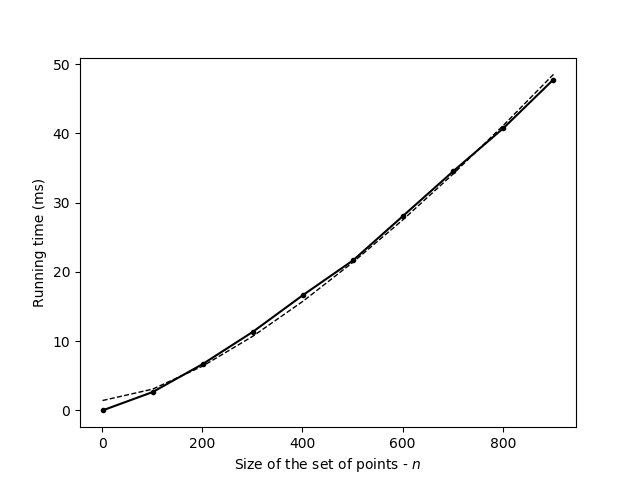
\includegraphics[width=0.6\textwidth]{range_tree_construction_performance}
        }{
            \caption{Performance of the range tree construction}
            \label{fig:range_tree_construction_performance}
        }
        \capbtabbox[0.3\textwidth][\FBheight][t]{
            \small
            \begin{tabular}{cc}
                Size $n$ & Running time (ms) \\
                \hline
                $1$ & 0.003 \\
                $101$ & 2.653 \\
                $201$ & 6.700 \\
                $301$ & 11.351 \\
                $401$ & 16.652 \\
                $501$ & 21.668 \\
                $601$ & 28.102 \\
                $701$ & 34.542 \\
                $801$ & 40.757 \\
                $901$ & 47.785
            \end{tabular}
        }{}
    \end{floatrow}
\end{figure}

\paragraph{Range tree search.} The range tree search is an $O(\log^3 n)$ operation. The results are presented in \figref{fig:range_tree_search_performance}. We derive a line of best fit $y = \alpha \log^3 n + \beta$ with $\alpha = 1.633 \times 10^{-2}$ and $\beta = 7.932 \times 10^{-1}$. This gives an empirical complexity of $t \sim 1.633 \times 10^{-2} \log^3 n + 7.932 \times 10^{-1}$, where $t$ denotes the running time. The empirical running time matches the theoretical bound of $O(\log^3 n)$.

\begin{figure}[h!]
    \begin{floatrow}
        \ffigbox[\FBwidth][\FBheight][t]{
            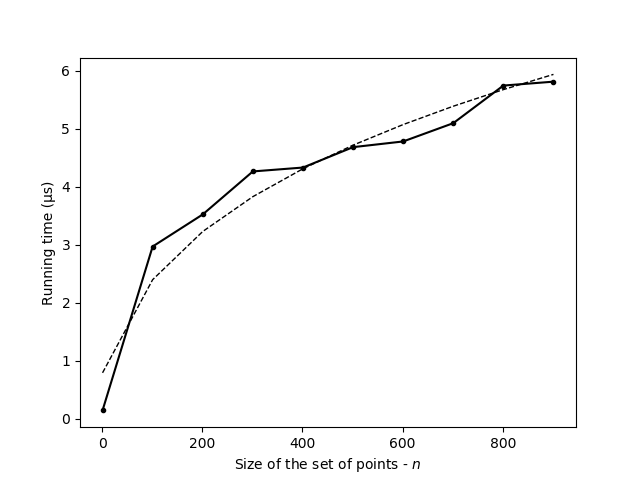
\includegraphics[width=0.6\textwidth]{range_tree_search_performance}
        }{
            \caption{Performance of the range tree search}
            \label{fig:range_tree_search_performance}
        }
        \capbtabbox[0.3\textwidth][\FBheight][t]{
            \small
            \begin{tabular}{cc}
                Size $n$ & Running time ($\mathrm{\mu}$s) \\
                \hline
                $1$ & 0.146 \\
                $101$ & 2.970 \\
                $201$ & 3.523 \\
                $301$ & 4.263 \\
                $401$ & 4.330 \\
                $501$ & 4.682 \\
                $601$ & 4.780 \\
                $701$ & 5.095 \\
                $801$ & 5.473 \\
                $901$ & 5.810
            \end{tabular}
        }{}
    \end{floatrow}
\end{figure}

\subsubsection{Tangent Computation}

The tangent computation, as described in \ref{subsub:tangent_computation}, is an $O(\log(a + b))$ subroutine, where $a$ and $b$ are the sizes of each polygon respectively. The tangent computation subroutine is tested on polygons of size $n = 2^k$ for each $k \in [0, 15]$. For each $k$, the two polygons of size $2^k$ are independently generated by taking $2^k$ random samples of the unit circle under uniform distribution. The results are presented in \figref{fig:tangent_computation_performance}. Empirically, the running time of the tangent computation is directly proportional to $\log_2(n)$. From the data, we derive a line of best fit $y = \alpha k + \beta$ with $\alpha = 64.273$ and $\beta = 14.939$. This gives an empirical complexity of $t \sim 64.273 \log_2 (n) + 14.939$, where $t$ denotes the running time. The empirical running time matches the theoretical bound of $O(\log(a+b))$.

\begin{figure}[h!]
    \begin{floatrow}
        \ffigbox[\FBwidth][\FBheight][t]{
            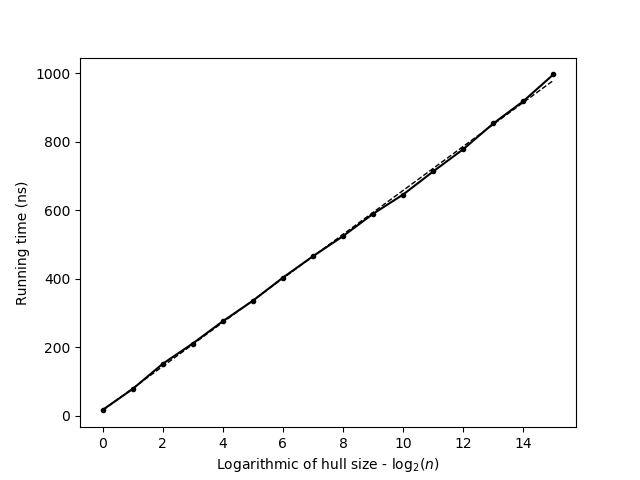
\includegraphics[width=0.6\textwidth]{tangent_computation_performance}
        }{
            \caption{Performance of the tangent computation}
            \label{fig:tangent_computation_performance}
        }
        \capbtabbox[0.3\textwidth][\FBheight][t]{
            \small
            \begin{tabular}{cc}
                $\log_2(n)$ & Running time (ns) \\
                \hline
                0 & 16.191 \\
                1 & 77.376 \\
                2 & 150.99 \\
                3 & 210.307 \\
                4 & 275.398 \\
                5 & 335.235 \\
                6 & 402.821 \\
                7 & 465.305 \\
                8 & 524.074 \\
                9 & 589.302 \\
                10 & 645.533 \\
                11 & 713.073 \\
                12 & 778.048 \\
                13 & 853.159 \\
                14 & 918.426 \\
                15 & 996.516
            \end{tabular}
        }{}
    \end{floatrow}
\end{figure}

\subsection{Designing Adversarial Inputs} \label{sub:designing_adversarial_inputs}

\subsubsection{Identifying the Performance Bottleneck}

In this section, we aim to identify the characteristics of ``adversarial inputs'', that is, inputs that impose a worst-case scenario on one or more subroutines of the algorithm. Recall from \figref{fig:hierarchy} that the $O(n\log^4n)$ overall running time of this algorithm is produced by $O(n)$ calls to the $O(\log^4 n)$ subroutine of \texttt{half\_plane\_intersects}, which can be further dissected into $O(\log^3 n)$ calls to the $O(\log n)$ tangent computation subroutine (\texttt{compute\_tangent}). Therefore, the critical chain for acheiving this $O(n \log^4 n)$ is as \figref{fig:tangent_dependencies}.

\begin{figure}[h!]
    \centering
    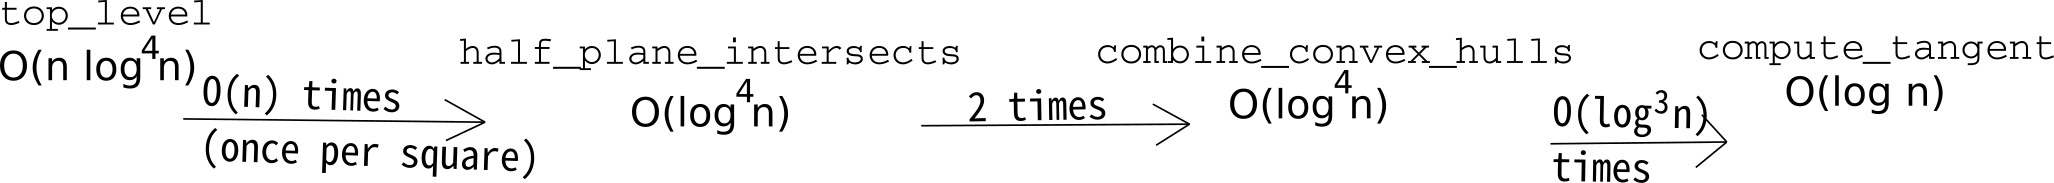
\includegraphics[width=0.9\textwidth]{images/tangent_computations_simplified.png}
    \caption{The critical chain for achieving $O(n \log^4 n)$ running time}
    \label{fig:tangent_dependencies}
\end{figure}

In the theoretical analysis by Abrahamsem et al. \cite{abb17}, the $O(\log^4 n)$ running time bound is given as a function of the input size $n$. Given a fixed $n$, the running time bound does not include any characterization of the distribution of the set of input points. Nonetheless, observe that in the tangent computation subroutine, the running time is a function of the sizes of each polygon, rather than the number of points contained within each polygon. Therefore, it is necessary for us to investigate how the distribution of points within a point set impacts the performance of the tangent computation subroutine, as well as the entire algorithm.

To be concrete, given a process of generating a point set $P$, we are interested in the expected complexity of $\CH(P)$ in terms of the number of points in $P$. We first formalize the process of generating a point set. Given a bounded convex set $\mathcal{R} \subset \mathbb{R}^2$, as well as the number of points $n$. A point set $P_\mathcal{R}^D$ is generated via $n$ independent random samples of $\mathcal{R}$ under distribution $D$. Let $h_\mathcal{R}(n)^D$ denote the expected size of $\CH(P)$. Efron \cite{efr65} showed that if the expected area of $\CH(P)$ is at least $(1-f(n)) \mathrm{Area}(\mathcal{R})$, where $1 \geq f(n) \geq 0$ for $n \geq 0$, then the expected size of $\CH(P)$ is at most $nf(n/2)$ under uniform distribution. Based on this result, Har-Peled \cite{hp11} showed that if $\mathcal{R}$ resembles a convex polygon with $k$ sides, then $h_\mathcal{R}^U = O(k \log n)$, where $U$ denotes a uniform distribution over $\mathcal{R}$. And if $\mathcal{R}$ resembles a disk, then $h_\mathcal{R}^U = O(n^{1/3})$. Based on these findings, we will attempt to design a worst-case input for a fixed point-set size $n$ selected via independent uniform samples over a convex region. We will then compare this result with the point set selected under normal distribution. For completeness, we will also include the extreme case, where all points lie on the convex hull of the point set.

\subsubsection{Uniform Random Sampling on a Disk}

We test the tangent computation subroutine with input sets derived by uniform random sampling on a disk. The tangent computation subroutine is tested on input set size $n = 2^k$ for each $k \in [0, 9]$. For each $k$, the two point sets of size $2^k$ are independently generated by taking $2^k$ random samples on a unit disk under uniform distribution. The results are presented in \figref{fig:uniform_disk_input}. Observe that sampling on a disk exhibits a sublinear pattern with respect to $\log_2(n)$, as compared to the linear pattern exhibited by sampling directly on a circle. This observation is qualitatively in line with the $O(n^{1/3})$ expected hull size by Har-Peled \cite{hp11}.

\begin{figure}[h!]
    \begin{floatrow}
        \ffigbox[\FBwidth][\FBheight][t]{
            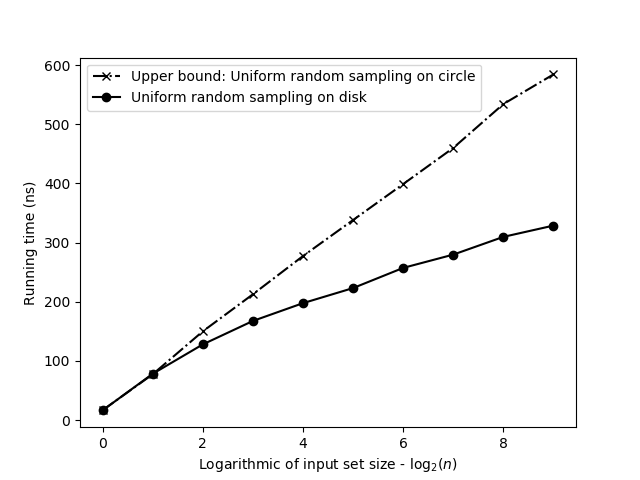
\includegraphics[width=0.6\textwidth]{uniform_disk_input}
        }{
            \caption{Performance of uniform random sampling on disk}
            \label{fig:uniform_disk_input}
        }
        \capbtabbox[0.3\textwidth][\FBheight][t]{
            \small
            \begin{tabular}{cc}
                $\log_2(n)$ & Running time (ns) \\
                \hline
                0 & 16.371 \\
                1 & 78.192 \\
                2 & 127.893 \\
                3 & 167.572 \\
                4 & 197.670 \\
                5 & 223.183 \\
                6 & 257.281 \\
                7 & 279.767 \\
                8 & 309.755 \\
                9 & 328.822
            \end{tabular}
        }{}
    \end{floatrow}
\end{figure}

\subsubsection{Uniform Random Sampling in a Polygon}

Next, we test the tangent computation subroutine with input sets derived by uniform random sampling in the area enclosed by a polygon. The tangent computation subroutine is tested on input size $n = 2^k$ for each $k \in [0, 9]$. For each $k$, the two point sets of size $2^k$ are independently generated by taking $2^k$ random samples in the area enclosed by a polygon under uniform distribution. For this test, regular polygons of $3$, $4$ and $5$ sides are used. The results are presented in \figref{fig:uniform_polygon_input} and \tabref{tab:uniform_polygon_input}. Observe that sampling in a polygon exhibits a sublinear pattern with respect to $\log_2(n)$. Addtionally, the running time increases as the number of sides $\gamma$ increases. These findings are in line with the $O(\gamma \log n)$ expected hull size by Har-Peled \cite{hp11}.

\begin{figure}[h!]
    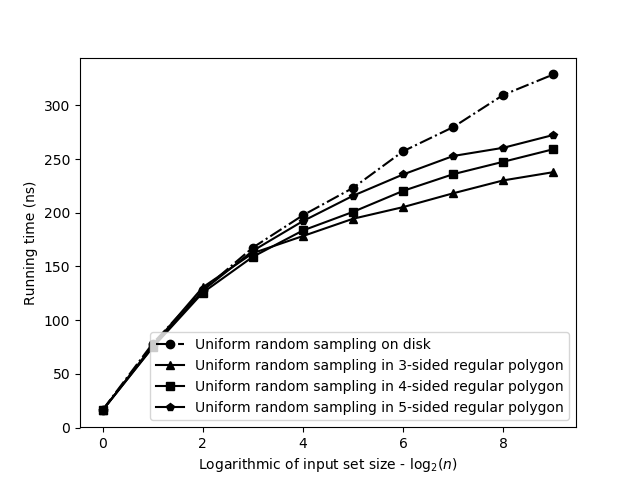
\includegraphics[width=0.6\textwidth]{uniform_polygon_input}
    \caption{Performance of uniform random sampling in polygons}
    \label{fig:uniform_polygon_input}
\end{figure}

\begin{table}[h!]
    \begin{tabular}{cccc}
        $\log_2(n)$ & 3-sided time (ns) & 4-sided time (ns) & 5-sided time (ns) \\
        \hline
        0 & 15.965 & 15.952 & 16.088 \\
        1 & 76.272 & 74.553 & 75.002 \\
        2 & 130.562 & 125.597 & 127.57 \\
        3 & 162.382 & 158.997 & 164.573 \\
        4 & 178.309 & 183.507 & 192.230 \\
        5 & 194.411 & 200.815 & 215.828 \\
        6 & 205.253 & 220.388 & 235.682 \\
        7 & 218.142 & 235.914 & 252.868 \\
        8 & 230.136 & 247.495 & 260.496 \\
        9 & 237.814 & 259.173 & 272.446
    \end{tabular}
    \caption{Performance statistics of uniform random sampling in polygons}
    \label{tab:uniform_polygon_input}
\end{table}

\subsubsection{Range Tree Queries}

\begin{figure}
    \centering
    \begin{subfigure}[b]{0.4\textwidth}
    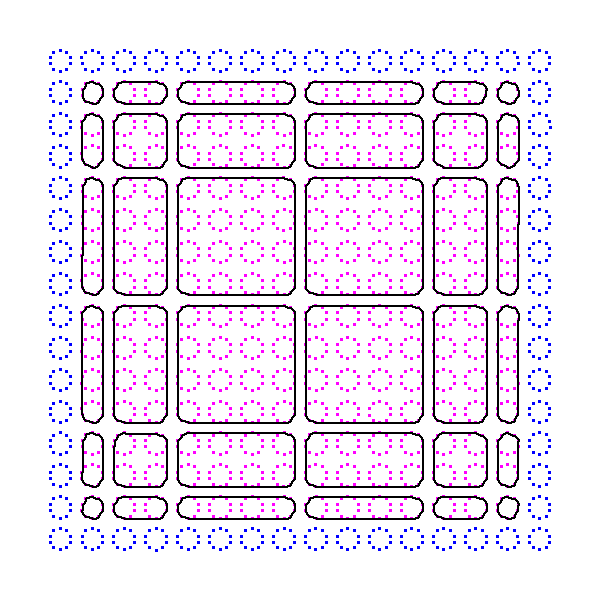
\includegraphics[width=\textwidth]{images/hard_tree_query.png}
    \end{subfigure}
    %
    \begin{subfigure}[b]{0.4\textwidth}
    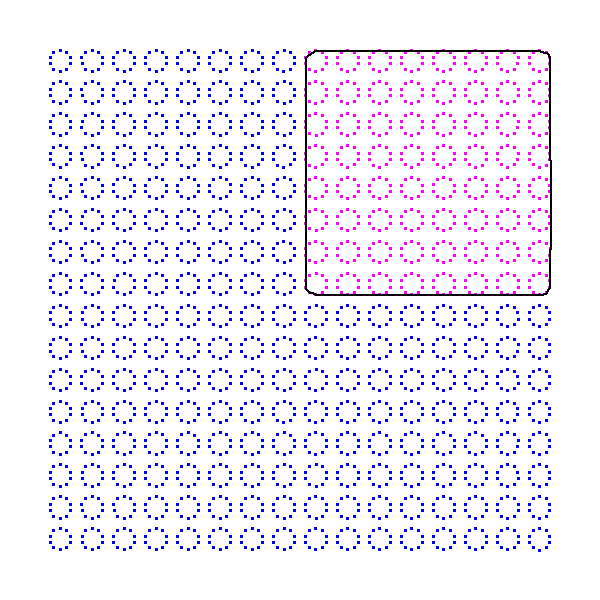
\includegraphics[width=\textwidth]{images/ok_input_range_tree.png}
    \end{subfigure}
    \caption{Left: A worst-case query to the range tree. Right: A best case query to the left tree.}
    \label{fig:range_queries}
\end{figure}

We have assumed that the number of input polygons to convex hull combination algorithm has been the worst case scenario - that is, $O(\log^3 n)$. We discuss briefly concerns about this assumptions.

In fact, a query to the range tree may leave as little as one input polygon. Figure \ref{fig:range_queries} shows the result from two range queries on axis-aligned windows on the same set of points. The best case is unlikely, as it requires the query region to exactly span a single subtree, of which there are only $O(n\log n)$, while the space of possible queries are $O(n^4)$ in two dimensions. The number of disjoint subtrees in each query is proportional with the number of queries resulting in that number of subtrees.

Thus, if we assume random construction of input queries, we can expect the the number of output polygons to be high. We would have to fully implement the quad tree construction to fully verify that this result is realistic.

\subsubsection{Conclusion} \label{subsub:polygon_convergence_to_disk}

Observe that as the number of sides $\gamma$ increases in a regular polygon of a given radius $r$, the polygon occupies an increasing proportion of area of a disk of radius $r$. The limit of this ratio is $1$ as $\gamma$ approaches infinity. By Har-Peled \cite{hp11}, the running time of the tangent computation subroutine increases monotonically as $\gamma$ increases. Therefore, the running time of the tangent computation in a $\gamma$-sided polygon under uniform sampling converges to the running time on a disk under uniform sampling. We may hereby conclude that the worst-case scenario for tangent computation under uniform sampling is when $\mathcal{R} \subset \mathbb{R}^2$ is a disk. In this case, the expected hull size is $O(n^{1/3})$, and the corresponding running time for tangent computation is $O(\log (n^{1/3}))$.

% \subsubsection{Adversarial Inputs: Point Clusters}
% 
% Applying the conclusion in \ref{subsub:polygon_convergence_to_disk}, we design a class of adversarial inputs via point clusters. Let the input point set $S$ of $n$ points be the union of clusters $\{C_1, C_2, \ldots, C_m\}$. The set of clusters constitute a partition of $S$. The center $c_i$ of each cluster $C_i$ is independently chosen in a disk sample region under uniform random distribution. The \textit{cluster radius} $r$ is defined as $r \equiv R / m$, where $R$ denotes the radius of the sample region, and $m$ denotes the number of clusters. The points are equally distributed across all clusters. The set of points for each cluster $C_i$ is generated via independent sampling on a disk region of radius $r$ centered at $c_i$. \figref{fig:cluster_5} shows an example point set generated with 1000 points and 5 clusters.
% 
% \begin{figure}[h]
%     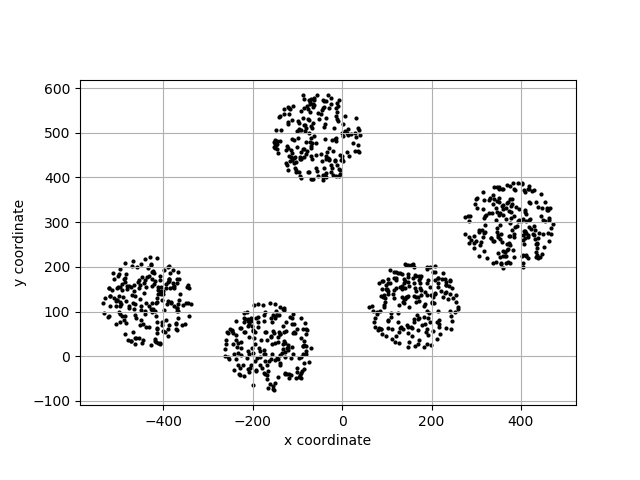
\includegraphics[width=0.6\textwidth]{cluster_5}
%     \caption{A point set generated with 1000 points and 5 clusters}
%     \label{fig:cluster_5}
% \end{figure}
% 
% Observe that the expected hull size for uniform random sampling on a disk is sublinear. Hence when the total number of points is a fixed value, in order to maximize the total running time of all tangent subroutines, we wish to maximize the number of polygons produced by the range tree search subroutine. Given a fix number of points $n$, we wish 

%\subsection{Input Generation via Gradient Descent}

% Experimental input generation

\section{Limitations} \label{sec:limitations}

After working with this algorithm, we have identified a couple of key issues concerning our implementation of the algorithm impacting the analysis, and practical use of the algorithm in general.

\subsection{RAM Usage}

As we described, the algorithm requires us (if we wish to withhold the best possible running time) to build and keep about $18000^2$ range trees in memories, one for each pair of the 18001 points, each such tree having size $O(n \log^3 n)$. An optimization that minimizes this number a little, is to exploit that many of the lines will be parallel: Since the range trees computed over the lines only depend on the angles of the lines, we can avoid many duplicate trees by pruning the ones corresponding to equal angles. A simple computation (see \texttt{/count\_unique\_line\_orientations} in \cite{hm18}) showed that the number of remaining unique line orientations was 63,431,423, which still means a huge memory consumption for large $n$.

\subsection{The Convex Hull Combining Procedure}

As mentioned before, we use a subroutine taking in $k$ convex hulls consisting of $m$ points in total. The paper claims that this subroutine runs in $O(k \log m)$ time. Our implementation of the routine, however, uses $O(m + k\log m)$ time, which shifts the total running time of the algorithm from $O(n \log^4 n)$ to $O(n^2)$ in the worst case.

The main problem is that our implementation computes each vertically sliced polygon explicitly, which automatically ramps up the running time to $O(m)$. We have failed to identify a proper way of implicitly storing these new polygons in a way that is also suitable for the subsequent tangent computations. 

\subsection{Lack of Quad Tree Construction}

As previously mentioned, we chose not to implement the quad tree, as we predicted it to not severely impact the running time. While it is true that the construction itself does not significantly contribute to the time usage, the set of squares $S$ in which the construction results, largely steers the queries issued to the range tree subsequently. Thus, our early decision of leaving out the implementation of this subroutine has, in hindsight, left us incapable of reliably creating realistic queries for the range trees.

\section{Conclusion} \label{sec:conclusion}

% Positive things we have explored / come across

In this implementation project, we analyzed the structure of the $O(n \log^4 n)$ minimum perimeter-sum bipartition algorithm by Abrahamsen et al. \cite{abb17}. The algorithm was studied as a collection of subroutines, and the structural hierarchy of these subroutines was established. This allowed us to implement the most important components of the algorithm and identify its performance bottleneck by analyzing the critical chain that supports its runtime bounds. For the basic subroutines that occupy leaf positions of the structural hierarchy, we showed that the empirical running times match their theoretical bounds, and obtained the degree $0$ and $1$ constant factors for the empirical running times.

By analyzing the critical chain, we identified the tangent computation subroutine as our target of adversarial input. We formalized the problem of generating the worst-case input for tangent computation as finding a convex sampling region that maximizes expected hull sizes of random polygons. We compared the performance of the tangent computation subroutine when sampled on regular polygons and disks, and concluded that the worst-case scenario occurs when the sampling region is a disk; in which case, the worst-case running time of the tangent computation subroutine is $O(\log(n^{1/3})$, where $n$ is the size of the input set.

% Not so positive things

A limiting factor to our analysis is that not all parts of the algorithm have been implemented. Although we were able to identify the basic subroutines from the structural hierarchy, we were not able to produce empirical results of the entire algorithm. This limitation has constrained our ability to fully understand the behavior of the algorithm on varying inputs.

\bibliographystyle{acm}
\bibliography{main}

\begin{appendices}
    \section{Specifications and Testing Methodology} \label{apdx:specifications}

    \subsection{Testing Environment}

    All performance testings in this report are completed on a single $4.7$GHz physical thread on an \texttt{x86-64} processor. The memory in use is of DDR4 at $3200$MHz (PC4 25600). Testing is completed under a virtualized instance of Arch Linux distribution via VT-d, with Linux kernel version \texttt{4.19.8} and \texttt{gcc} version \texttt{8.2.1 20181127}.

    \subsection{Testing Methodology}

    The testing methodologies applied for each subroutine are listed as follows:

    \subsubsection{Outer Triangle Partitioning}

    In performance testing, given target size $n$, the point set of size $n$ is generated as follows:
    \begin{enumerate}
        \item Define the center of the sampling region as $(0, 0)$.
        \item Define the sampling region to be a disk of radius $500$.
        \item Points are selected via uniform sampling over the disk region via the discard method.
    \end{enumerate}
    For each given $n$, we generate $10^2$ random point sets. For each point set, the outer triangle partitioning operation is performed once. The result is obtained via averaging these samples.

    \subsubsection{Range Tree Construction and Search}

    In performance testing, given target size $n$, the point set of size $n$ is generated as follows:
    \begin{enumerate}
        \item Define the sampling region as a square of side length $1000$ defined by the following vertices: $(500, 500)$, $(500, -500)$, $(-500, 500)$, $(-500, -500)$.
        \item Points are selected via uniform random sampling over the sampling region. 
    \end{enumerate}
    Additionally, the following definitions are used:
    \begin{enumerate}
        \item The vector perpendicular to the $x$-$y$ separator halfplane (\texttt{halfplane\_dir}) is defined to be $(1, 1)$.
        \item The region of the range tree query is defined to be the square on the following vertices: $(500, 500)$, $(500, -500)$, $(-500, 500)$, $(-500, -500)$.
        \item The comparator point is defined to be $(0, 0)$.
    \end{enumerate}
    For the construction test, we generate $10^1$ random point sets. For each point set, the range tree construction operation is performed once. For the search test, we generate $10^1$ random point sets. For each point set, the range tree construction operation is performed $10^5$ times. The result is obtained via averaging in each category.

    \subsubsection{Tangent Computation}

    In performance testing, given convex hull complexity $k$, the pair of polygons is generated as follows:
    \begin{enumerate}
        \item Define the center of the left polygon as $(-1000, 0)$, and the center of the right polygon as $(1000, 0)$.
        \item For each polygon, define a circle of radius $500$ with its respective center.
        \item For each polygon, generate $\theta \in [0, 2\pi)$ via random sampling. Find the point on the polygon's circle that corresponds to $\theta$. Repeat this process $k$ times. A size $k$ point set via independent uniform sampling on the circle is thus generated. Observe that the convex hull of this point set would have size exactly $k$. 
    \end{enumerate}
    We generate $10^3$ random pairs of polygons following this methodology. For each pair of polygons, the tangent computation is performed $10^6$ times. The result is obtained via averaging these samples. 

    In input analysis, given convex point set size $n$ and distribution $D$, the pair of point sets is generated as follows:
    \begin{enumerate}
        \item Define the center of the left sampling region as $(-1000, 0)$, and the center of the right sampling region as $(1000, 0)$.
        \item For each sampling region, we identify a bounding box of the sampling region, and apply the distribution $D$ on the bounding box, and generate the point sets via the discard method. Specifically,
        \begin{enumerate}
            \item If the sampling region is a regular polygon, we define its radius, that is, the distance from its center to any of its vertices, to be $500$.
            \item If the sampling region is a disk, we define its radius to be $500$.
            \item If the sampling region is a circle (for the degenerate extreme case), sampling is performed in the same way as in performance testing.
        \end{enumerate}
    \end{enumerate}
    We generate $10^3$ random pairs of point sets following this methodology. For each pair of point sets, the tangent computation is performed $10^5$ times. The result is obtained via averaging these samples.
\end{appendices}

\end{document}
